%\newcommand{\EQ}{\kw{EQ}}
\newpage
\addtolength{\parskip}{0.25cm}
\newpage
\section*{\Large \sf APPENDIX-cp}
\label{sec-proofs}



\subsection{Optimization Techniques for Algorithm \grouprec}.
%
\begin{figure}[tb!]
\vspace{2ex}
\begin{center}
{\small

\myhrule \vspace{-2ex}
\mat{0ex}{
\sstab {\sl Input:\/} Pattern graph $P(V_p$, $E_p$, $l_p$, $f_p)$.\\
{\sl Output:\/} A minimum equivalent pattern graph $P_m$ of $P$.\\
\bcc \quad if $P$ is not a consistent pattern graph then return null.\\
\icc \quad Compute the maximum match relation $S$ of $P \eps P$;\\
\icc \quad Compute equivalent classes of nodes in $P$ based on $S$;\\
\icc \quad Create a node for each equivalent class in $P_m$;\\
\icc \quad Connect different equivalent classes by necessary edges in $P_m$;\\
\icc \quad Compute the intersection of interval bounds on pattern nodes in \\each equivalent class and put on the corresponding node in $P_m$;\\
\icc return $P_m$;\\
}
\vspace{-2.5ex}

\myhrule
}
\end{center}
\vspace{-4ex}
\caption{minP} \label{minP-alg}
\vspace{-3ex}
\end{figure}

%
We next present optimization techniques for algorithm \grouprec, by means of query minimization, as stated below, yielding the optimization algorithm \grouprecopt.

Query minimization is important for any query language. Minimizing pattern graphs is an effective way for improving the efficiency of querying data graphs. By Proposition~\ref{prop-pattern-consistency}, a pattern graph can be determined whether is satisfiable or not in quadratic time. Once we know a pattern graph is consistent, the $r$-simulation computing process can be optimized by minimizing the pattern graphs.

We say two pattern graphs $P$ and $P'$ are {\em equivalent via $r$-simulation}, denoted by $P\equiv P'$, iff for any data graph $G$, $P(G) = P'(G)$ via $r$-simulation. We say $P$ is {\em minimum} if for any other pattern graph $P'$ such that $P\equiv P'$, $|P|\leq |P'|$.

\eat{
\begin{theorem}
\label{thm-pattern-minimization-ap}
For any pattern graph $P$ and radius $r$, (1) there exists a unique minimum equivalent pattern graph $P_m$, via $r$-simulation with, that finds the same maximum match relation on any data graph; (2) taking the intersection of interval bounds on pattern nodes in each equivalent class in $P_m$, and putting it on the corresponding pattern node in $P_m$, $P$ and $P_m$ are equivalent via $r$-simulation; and (3) there exists a quadratic time algorithm to find its minimum equivalent pattern graph.
\end{theorem}
}

\begin{theorem}
\label{thm-pattern-minimization-ap}
For any pattern graph $P(V_p, E_p)$ and radius $r$, (1) there exists a unique minimum equivalent pattern graph $P_m$ via $r$-simulation;
and (2) there exists an algorithm that finds $P_m$ in $((|V_p|+|E_p|)^2)$ time.
\end{theorem}


\eat{
\stitle{Remarks}.
(1) A pattern graph $P$ may have multiple minimum equivalent pattern graphs $P_m^1$, $P_m^2$,..., $P_m^k$, of the same size but are not isomorphic to each other. Their structures must be exactly same, while the capacity on the corresponding nodes may be different, but they still return the same match result on any data graph.
%
(2) There exists method to get a unique minimum equivalent pattern graph, which takes linear time. Is unifying step necessary? Adopt or not?
}

\etitle{Algorithm \minp} As a proof of Theorem~\ref{thm-pattern-minimization}, we present Algorithm \minp to minimize pattern graphs as shown in Fig.~\ref{minP-alg}. It takes as input a pattern graph $P$, and outputs a minimum equivalent pattern graph $P_m$ of $P$ via graph simulation and some capacity bound computing. For any pattern graph $P$, it first checks to see whether $P$ is consistent. If the answer is yes, it then executes the following minimization steps. In the minimization process, It first computes the maximum match relation $R$ by treating $P$ as both a pattern and a data graph(line 2). It then computes equivalent classes for nodes in $P$ such that $u$ and $v$ are in the same class iff both $(u, v)\in R$ and $(v, u)\in R$ (line 3). Finally, it constructs the minimum equivalent pattern graph $P_m$ as follows (lines 4-6).(a) For each equivalent class \kw{eq}, it creates a node \kw{eq} for $P_m$; (b) there is an edge (\kw{eq}, \kw{eq'}) in $P_m$ iff there exist nodes $u \in \kw{eq}$ and $u' \in \kw{eq'}$ such that there is an edge $(u, u')$ in $P_m$; and (c) it computes the intersection of capacity bounds on pattern nodes in each equivalent class \kw{eq} and put on the corresponding node \kw{eq} in $P_m$.


\eat{%%%%%%%%%%%EAT
\begin{figure}[tb!]
\vspace{-2ex}
\begin{center}
{\small

\myhrule \vspace{-2ex}
\mat{0ex}{
\sstab {\sl Input:\/} Pattern graph $P(V_p$, $E_p$, $l_p$, $f_p)$.\\
{\sl Output:\/} A minimum equivalent pattern graph $P_m$ of $P$.\\
\bcc \quad if $P$ is not a consistent pattern graph then return null.\\
\icc \quad Compute the maximum match relation $R$ of $P \eps P$;\\
\icc \quad Compute equivalent classes of nodes in $P$ based on $R$;\\
\icc \quad Create a node for each equivalent class in $P_m$;\\
\icc \quad Connect different equivalent classes by necessary edges in $P_m$;\\
\icc \quad Compute the intersection of interval bounds on pattern nodes in \\each equivalent class and put on the corresponding node in $P_m$;\\
\icc return $P_m$;\\
}
\vspace{-2.5ex}

\myhrule
}
\end{center}
\vspace{-4ex}
\caption{\minp} \label{minP-alg}
\vspace{-3ex}
\end{figure}
}%%%%%%%%%%%%%EAT

\begin{example}
Takes as input the pattern graph $P_3$ given in Fig.~\ref{fig-consistency-example}. Algorithm works as follows. By Proposition~\ref{prop-pattern-consistency}, it determines that $P_3$ is a consistent pattern graph. In the minimization process, it first computes the maximum match relation $S$ by taking $P_3$ as both pattern and data graph, producing $S$ = \{$(A, A)$, $(B_1, B_2)$, $(B_2, B_1)$, $(C_i, C_j)$\} ($i,j \in [1,3]$). It then computes three equivalent classes: $\kw{eq_A}$=\{$A$\}, $\kw{eq_B}$=\{$B_1, B_2$\}, and $\kw{eq_C}$=\{$C_1, C_2, C_3$\}. Finally, it constructs the minimum equivalent pattern graph $P_m$ of $P$, as shown in Fig.~\ref{fig-consistency-example}. (a) For each equivalent class $\kw{eq_A}$, $\kw{eq_B}$ and $\kw{eq_C}$, it creates node labeled with $A$, $B$, and $C$ respectively; (b) it creates an edge $(A,B)$ connecting the class nodes of $\kw{eq_A}$ and $\kw{eq_B}$ in $P_m$, as there exists an edge $(u,v)$ in $P_3$ with $u \in \kw{eq_A}$ and $v \in \kw{eq_B}$, the same for edge $(B,C)$; and (c) for equivalent class $eq_B$, it computes the intersection of interval bounds on pattern nodes in it, that is, $[1,3]\cap[2,5] = [2,3]$, and [1,1], [3,4] for $eq_A$, $eq_C$. At last it puts them on the corresponding nodes in $P_{3m}$.
\end{example}

\etitle{Correctness and Complexity}. The correctness of Algorithm \minp is assured by the following. (1) $P_m \equiv P$, ensuring they return exactly the same result on any data graph; and (2) $P_m$ is minimum in size, \ie there is no other equivalent query $P'$ smaller than $P_m$.

Algorithm minP is in $O((|V_p|+|E_p|)^2)$ time. Indeed, step 1 (line 2), 2 (line 3), 3 (line 4-5) and 4 (line 6) of minP take $O((|V_p|+|E_p|)^2)$ time, $O(|V_p|^2)$ time, $O(|E_p|)$ time and $O(|V_p|^2)$ time, respectively.

Besides, algorithm \grouprecopt builds balls only using the set of data nodes with labels included in pattern nodes, instead of using all data nodes, which is an effective improvement for algorithm \grouprec.

\eat{
\stitle{Algorithm $\incgrpat^+$}

\begin{figure}[hb!]
\vspace{-2ex}
\begin{center}
{\small

\myhrule \vspace{-2ex}
\mat{0ex}{
\sstab {\sl Input:\/} Pattern graph $Pt_i(V_{Pt_i}$, $E_{Pt_i})$, data ball $\ball{w,r}$, $mat_i(\cdot)$,\\ and an edge $e=(u,u')$ to be inserted into $Pt_i$.\\
{\sl Output:\/} The updated match relation $mat_i(\cdot)$.\\
\bcc \quad $AFNode:=\emptyset$;\\
\icc \quad for each node $v \in mat_i(u)$ do\\
\icc \quad\quad if there is no $v' \in mat_i(u')$ with $(v, v')\in V_{\hat{G}}$\\
\icc \quad\quad then $AFNode:=AFNode \cup \{v\}$;\\
\icc \quad for each node $v' \in mat_i(u')$ do\\
\icc \quad\quad if there is no $v \in mat_i(u)$ with $(v', v)\in V_{\hat{G}}$\\
\icc \quad\quad then $AFNode:=AFNode \cup \{v'\}$;\\
\icc \quad for each node $v \in AFNode$ do\\
\icc \quad\quad $wSet:=\emptyset$;\\
\icc \quad\quad for each adjacent edge $(v,v')$ of $v$ do\\
\icc \quad\quad\quad for all $(u,u')\in E_p$ having $v \in mat_i(u)$ and $v'\in mat_i(u')$ do\\
\icc \quad\quad\quad\quad if $adjacent(l_p(u),v')\cap mat_i(u)=\emptyset$ then\\
\icc \quad\quad\quad\quad\quad $wSet$.push($(u',v')$);\\
\icc \quad\quad\quad\quad\quad while ($wSet\neq \emptyset$) do\\
\icc \quad\quad\quad\quad\quad\quad $(u',v'):=wSet$.pop();\\
\icc \quad\quad\quad\quad\quad\quad $mat_i(u')=mat_i(u')\backslash\{v'\}$;\\
\icc \quad\quad\quad\quad\quad\quad for all $(u',u'')\in E_p$ do\\
\icc \quad\quad\quad\quad\quad\quad\quad for all $v''\in adjacent(l_p(u''),v')\cap mat_i(u'')$ do\\
\icc \quad\quad\quad\quad\quad\quad\quad\quad if $adjacent(l_p(u'),v'')\cap mat_i(u')=\emptyset$ then \\
\icc \quad\quad\quad\quad\quad\quad\quad\quad\quad $wSet$.push($(u'',v'')$);\\
\icc if there is a pattern node $u$ having $|mat_i(u)| = 0$ then $mat_i=\emptyset$\\
\icc return $mat_i(\cdot)$;
}

\vspace{-2.5ex} \myhrule
}
\end{center}
\vspace{-4ex}
\caption{$\incgrpat^+$} \label{incpat-unit-insert}
\vspace{-3ex}
\end{figure}
}



\stitle{Linear $2$-approximation for density upper bounding}.
Given a ball $\ball{v,r}$ in $G$ and a pattern $P$, it computes density bound $ub$ to the perfect graph $\hat{G}_s$ of $P$ in $\ball{v,r}$ in $O(|\ball{v,r}|)$ time, such that $\kw{den}(\hat{G}_s) \leq d_{\kw{max}} \leq ub$, where $\kw{den}(\hat{G}_s)$ is the density of $\hat{G}_s$ and $d_{\kw{max}}$ is the density of the densest subgraph of $\ball{v,r}$.
Therefore, we can treat $ub$ as an upper bound on the density of $\hat{G}_s$. More specifically, it computes the $ub$ in three steps, as follows.

\sstab (1) Filter out to get a subgraph $\hat{G}_P$ from ball $\ball{v,r}$ such that $\hat{G}_P$ contains nodes with labels appeared in $P$ only, and the induced edges, in $O(|\ball{v,r}|)$ time.

\sstab (2) Compute the density $d$ of the {\em maximum core} of $\hat{G}_P$ in $O(|\hat{G}_P|)$ time.

\sstab (3) Return $2d$ as the density upper bound for $\hat{G}_s$ in $\ball{v,r}$.

Here the maximum core of a graph $G$ is defined as follows~\cite{EVMK12}.
A $l$-core of a graph $G$ is a subgraph $G_l$ of $G$ such that, each node in $G_l$ has degree no smaller than $l$.
A maximum core of a graph $G$ is a $l$-core $G_l$ of $G$ such that, for any non-empty $l'$-core $G_{l'}$ of $G$, $l'\leq l$. It is known that the maximum core of a graph $G$ can be computed in $O(|G|)$ time.

The following result ensures the above linear time algorithm returns $ub$ with the property claim above.

\begin{prop}
\label{prop-approximation-bound}
Given a graph $G$, let $d$ be the density of the maximum core of $G$, and $d_{\kw{max}}$ is the density of the densest subgraph of $G$, then $d\leq d_{\kw{max}} \leq 2d$.
\end{prop}



\subsection{NP-hardness}

We first formulate the {\em optimal $m$-fragmentation problem} ($\kw{OFGP}(P,m)$) as a bi-criteria optimization problem as follows.
\bi
\item Input: pattern graph $P$, an integer $m$.
\item Output: an $m$-fragmentation ${\cal P}_{m}$ composed of ${Pf}_1$, \ldots, ${Pf}_m$ and $F$ of $P$ such that (a) $\max_i |{Pf}_i|$ = $\max_i (|V_{{Pf}_i}| + |E_{{Pf}_i}|)$ is minimized; and (b) $|F|$ is minimized.
\ei
%Here $w(u)$ (resp. $w(e)$) is to represent the probability that a pattern update was applied to node $u$ (resp. edge $e$) in, \eg history pattern update workload, and can be set to 1 if no historical information is known.
That is, the problem is to implement the ``divide and conquer'' incremental strategy of the framework by finding a good $m$-fragmentation ${Pf}_1$, \ldots, ${Pf}_m$ and $F$ of the pattern graph such that
(i) the chances of the fragments ${Pf}_i$ to be updated are roughly the same, which further guarantees that the update time on any pattern fragment ${Pf}_i$ will be roughly equal, and the update time in all fragments is also minimized; and
(ii) the size of $F$ is also minimized such that the combination cost is minimized.

The decision version of $\kw{OFGP}(P, m)$, denoted by $\kw{dOFGP}(P, m, r_1, r_2)$, is to decide whether there exists a fragmentation ${Pf}_1$, \ldots, ${Pf}_m$ and $F$ such that, (a) $\max_i |{Pf}_i| \leq r_1\cdot\frac{|P|}{m}$ and (b) $|F|\leq r_2|P|$.
The corresponding single-criteria {\em cut}-minimization (resp. {\em fragment}-minimization) problem of $\kw{OFGP}(P, m)$, denoted by $\kw{OFFGP}(P, m, r)$ (resp. $\kw{OPFGP}(P, m, r)$), is to find an $m$-fragmentation ${Pf}_1$, \ldots, ${Pf}_m$ and $F$ such that $\max_i |{Pf}_i| \leq r\cdot\frac{|P|}{m}$ (resp. $|F|\leq r\cdot |P|$) and $|F|$ (resp. $\max_i |{Pf}_i|$) is minimized.

The problems are hard, as shown below.

\begin{prop}
\label{thm-fragmentation-hardness}
(1) $\kw{dOFGP}(P, m, r_1, r_2)$ is \NP-complete. It remains \NP-hard even $m$ = 2.

\sstab (2) Both $\kw{OFFGP}(P, m, r)$ and $\kw{OPFGP}(P, m, r)$ are \NPO-hard.
\end{prop}

Here \NPO is the class of all \NP optimization problems. An
\NPO-complete problem is \NP-hard to optimize, and is among the
hardest \NP optimization problems.

\begin{proofS}
(1) We show $\kw{dOFGP}$ is in \NP by giving an \NP algorithm that first guesses an $m$-cut $F$, and then check whether it divides $P$ into an $m$-fragmentation ${Pf}_1$, \ldots, ${Pf}_m$ such that $\max_i |{Pf}_i| \leq r_1\frac{|P|}{m}$ and $|F|\leq r_2|P|$. We show it is \NP-hard by reduction from the {\sc Minimum Bisection} problem, which is known \NP-hard even when $k=2$.
(2) We shown both $\kw{OFFGP}(P, m, r)$ and $\kw{OPFGP}(P, m, r)$ are \NPO-hard by proving that it is \NP-hard to decide whether there exists a feasible solution to both of them ({\bf To be verified}).
Indeed, there is no polynomial time approximation algorithm can guarantee a finite approximation ratio for $\kw{OFFGP}(P,m,r=1)$~\cite{AndreevR06}.
\end{proofS}


In light of Theorem~\ref{thm-fragmentation-hardness}, we give a heuristic algorithm, denoted by \kw{PFrag} and shown in Fig.~\ref{alg-PFrag}, for $\kw{OFGP}(P,m)$.
Algorithm \kw{PFrag} works by connecting $\kw{OFGP}(P,m)$ to the {\sc $(k, \nu)$-Balanced Partition} problem, which is to divided the vertices of a graph into $k$ components such that each component is of size more than $\nu\cdot\frac{n}{k}$, so that the number of edges between different compopents is minimized. The $(k,\nu)$-balanced partition problem, though is not approximable in general, has a number of sophisticated heuristic algorithms~\cite{AndreevR06}.

%%%%%%%%%%%%%%%%%%%%%Algorithm PFrag
\begin{figure}[t]
\begin{center}
{\small
\begin{center}
\myhrule \vspace{-2ex}
\mat{0ex}{
\sstab {\sl Input:\/} \= Pattern graph $P$, integer $m$.\\
{\sl Output:\/} An $m$-fragmentation ${Pf}_1$, \ldots, ${Pf}_m$, $F$ of $P$.\\
\stab \bcc \hspace{0.5ex} \= $k$ = $m$; $\nu$ = $m$; $M_P$ = $|P|$; $M_F$ = 0;\\
\icc \> $({Pf}^\nu_1, \ldots, {Pf}^\nu_m, F^\nu)$ := $\kw{BalanceP}(k,\nu)$; \\
\icc \> $M^\nu_P$ := $\kw{max}\{|{Pf}^\nu_1|, \ldots, |{Pf}^\nu_m|\}$; $M^\nu_F$ = $|F^\nu|$;\\
\icc\> \While $\kw{max}\{M_P, M_F\} > \kw{max}\{M^\nu_P, M^\nu_F\}$ \Do\\
\icc \>\hspace{2ex}\= ${Pf}_1$ := ${Pf}^\nu_1$, \ldots, ${Pf}_m$ := ${Pf}^\nu_m$;\\
\icc \>\hspace{2ex}\= $F$ := $F^\nu$; $M_P$ := $M^\nu_P$; $M_F$ := $M^\nu_F$;\\
\icc \>\> \If $M^\nu_P \geq M^\nu_F$ \Then $\nu := \frac{\nu}{2}$ \Else $\nu := \frac{3\nu}{2}$;\\
\icc \>\> $({Pf}^\nu_1, \ldots, {Pf}^\nu_m, F)$ := $\kw{BalanceP}(k,\nu)$;\\
\icc \>\> $M^\nu_P$ := $\kw{max}\{|{Pf}^\nu_1|, \ldots, |{Pf}^\nu_m|\}$; $M^\nu_F$ = $|F^\nu|$;\\
\icc \> \Return ${Pf}_1$, \ldots, ${Pf}_m$, $F$;
}
\vspace{-2.5ex} \myhrule
\end{center}
}
\end{center}
\vspace{-4ex}
\caption{Algorithm \kw{PFrag} \label{alg-PFrag}}
\vspace{-3ex}
\end{figure}


Given a pattern $P$ and an integer $m$, algorithm \kw{PFrag} finds an $m$-fragmentation for $P$ by recursively invoking algorithm $\kw{BalanceP}(k,\nu)$ for the {\sc $(k,\nu)$-Balanced partition} problem with different $\nu$, such that the final returned $m$-fragmentation strikes a balance between the size of each fragment ${Pf}_i$ of $P$ and the size of the cut $F$.
More specifically, \kw{PFrag} maintains $M_P$ and $M_F$ as the size of the maximum fragment of ${Pf}_i$  and the size of the cut in the $m$-fragmentation, respectively. Initially, it sets $M_p$ to $|P|$ and $M_F$ to 0 (line~1).
It then invokes \kw{BalanceP} with both $k$ and $\nu$ being $m$, \ie has no constraints on the size of fragments of $P$ (line~2).
After that, it iteratively checks whether the generated $m$-fragmentation can be improved (line~4) by adjusting $m$ in a {\em binary search style} (lines~4-9). If the current size of maximum fragment $M^\nu_P$ is no smaller than the size $M^\nu_F$ of the cut, it invokes \kw{BalanceP} with $m$ and $\frac{\nu}{2}$, and with $m$ and $\frac{3\nu}{2}$ otherwise (line~7). It returns the $m$-fragmentation if it cannot be improved anymore in this way (line~10).

\stitle{Correctness \& Complexity}.
The correctness is obvious as \kw{PFrag} always returns $m$-fragmentations.
Algorithm~\kw{PFrag} runs in $O(\log m\cdot t_{\kw{BalanceP}})$ time, where $t_{\kw{BalanceP}}$ is the complexity of the algorithm for the {\sc $(k,\nu)$-Balanced Partition} problem. Indeed, \kw{PFrag} calls at most $\log m$ times \kw{BalanceP}.\\

\stitle{Remark}. Given pattern $P$, an $m$-fragmentation ${\cal P}_{m}$ of $P$, a data
graph $G$ and $\tilde{M}(P,G)$, one can construct \matchindex of $O(2^{m} + |V|)$ bits
 within $O(|V|)$ time.


\subsection{Proof of Proposition~\ref{thm-inc-grouprec-pat}}


\begin{figure}[tb!]
\label{fig-inc-complexity-data}
\begin{center}
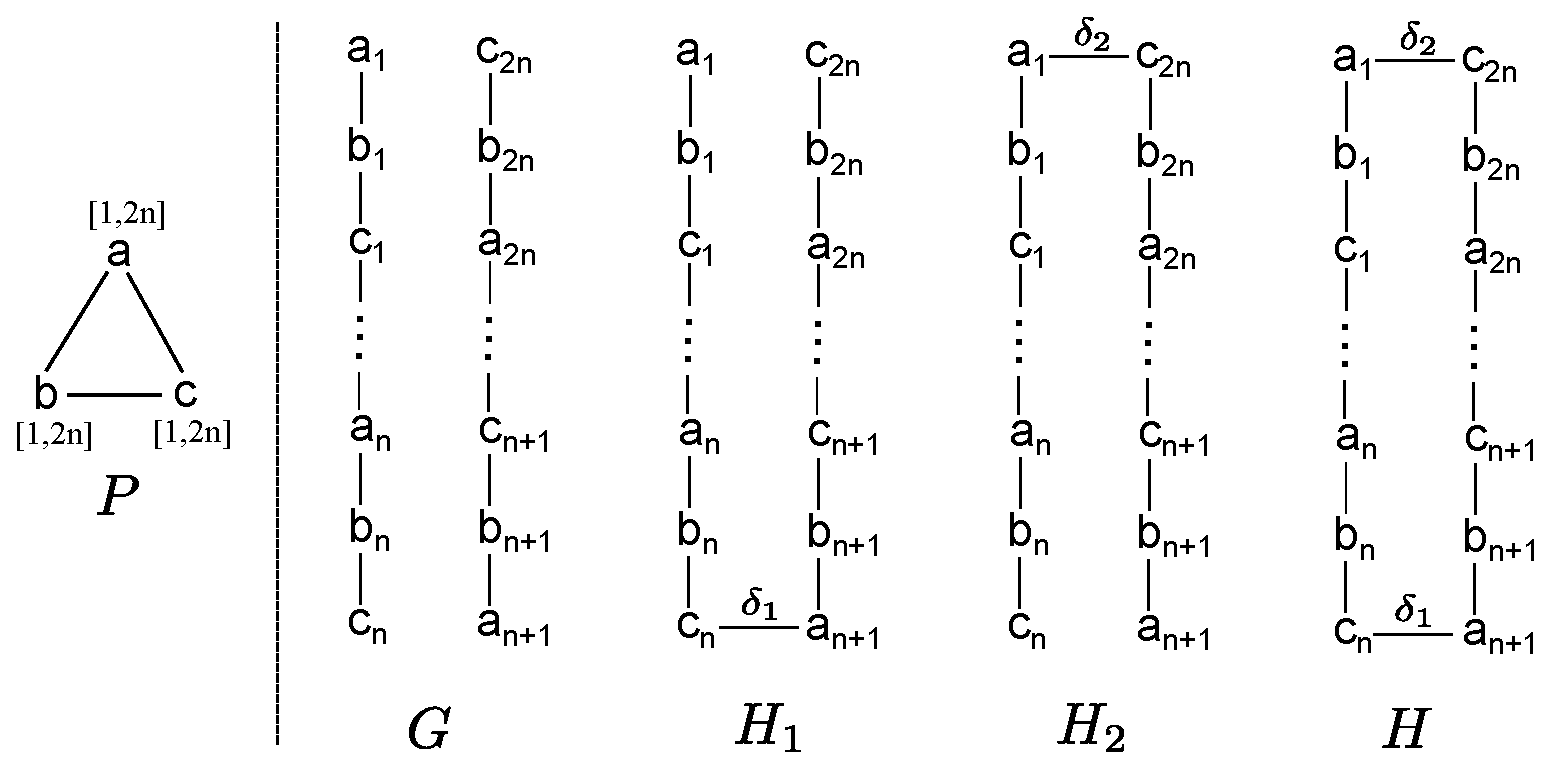
\includegraphics[scale=0.3]{./fig/inc-complexity-proof-data.eps}
\end{center}
\vspace{-3ex}
\caption{Unboundedness of single data update}
\vspace{-5ex}
\end{figure}

To show the unboundedness, we need to define what is an allowed algorithm to be discussed.  Here we adopt the notion of LP (locally persistent) graph algorithms \cite{Reps96} for proving unboundedness of graph algorithms.

The proof strictly follows the one in \cite{Reps96}.

\etitle{(1) \dyngr is unbounded for single data update}.
Following \cite{Reps96, FanWW13-tods}, consider the following pattern and data graphs, and single data updates. Let data graph $G$ consist of two chains ($a_1$, $b_1$, $c_1$, \ldots, $a_n$, $b_n$, $c_n$) and ($a_{n+1}$, $b_{n+1}$, $c_{n+1}$, \ldots, $a_{2n}$, $b_{2n}$, $c_{2n}$) where $a_i$, $b_i$ and $c_i$ have labels $A$, $B$ and $C$ respectively. Let pattern graph be a triangle with nodes $a$, $b$ and $c$ (labels are $A$, $B$ and $C$ respectively). Consider two single-edge insertions $\delta_1$ = ($c_n$, $a_{n+1}$) and $\delta_2$ = $(c_{2n}, a_1)$. Let $k = 1$ and $r$ = $6n$. Let $H_1$ and $H_2$ denote the graphs $G\oplus \delta_1$ and $G\oplus \delta_2$, respectively. Obviously, $PG_1(P, G) = PG_1(P, H_1) = PG_1(P, H_2) = \emptyset$, while $PG_1(P, H_1\oplus \delta_2) \neq \emptyset$. Assume that there exists a locally persistent incremental algorithm ${\cal A}$ for \dyngr. Let $Trace(G', \delta')$ denote the sequence of steps executed by the algorithm in processing some change $\delta'$ to some graph $G'$. Now consider the following two instances: the application of update $\delta_2$ to $G$ and the application of update $\delta_2$ to graph $H_1$. Obviously, the update procedure must behave differently in these two cases, and $Trace(G, \delta_2)$ must be different from $Trace(H_1, \delta_2)$ (because many vertices of $H_1\oplus \delta_2$ are affected, while no node in $G\oplus \delta_2$ is affected). Since a locally persistent algorithm makes use of no global storage, this can happen only both $Trace(G, \delta_2)$ and $Trace(H_1, \delta_2)$ include a visit to some node $w$ that contains different information in the graphs $G$ and $H_1$. However, $H_1$ was obtained from $G$ by applying change $\delta_1$. Hence the information at node $w$ must have been changed during the updating of applying $\delta_1$ to $G$. Therefore, $Trace(G, \delta_1)$ must also contain a visit to node $w$. As a characteristic of locally persistent algorithms is that if a vertex $w$ is visited during the updating of applying change $\delta'$ to graph $G'$, then every node in some path in $G'$ from a modified node of $\delta'$ to $w$ must have been visited.
Therefore, $Trace(G, \delta_1)$ and $Trace(G, \delta_2)$ both contain a visit to $w$, from the nodes in $\delta_1$ and $\delta_2$, respectively. Thus, $Trace(G, \delta_1)$ and $Trace(G, \delta_2)$ include visits to every node on some path from $c_n$ or $a_{n+1}$ to $c_{2n}$ or $a_1$ respectively. Hence, the time taken for processing change $\delta_1$ to $G$ plus the time taken for processing change $\delta_2$ to $G$ must be no smaller than the distance between $c_n$ or $a_{n+1}$ to $c_{2n}$ or $a_1$, \ie $n$, which is not a constant.
However, $|\kw{AFF}|$ in both cases are 1. Thus, the algorithm is not a bounded locally persistent incremental algorithm, which contradicts the assumption. That is, \dyngr is unbounded even for $k=1$ and single data update.


\begin{figure}[tb!]
\label{fig-inc-complexity-pattern}
\begin{center}
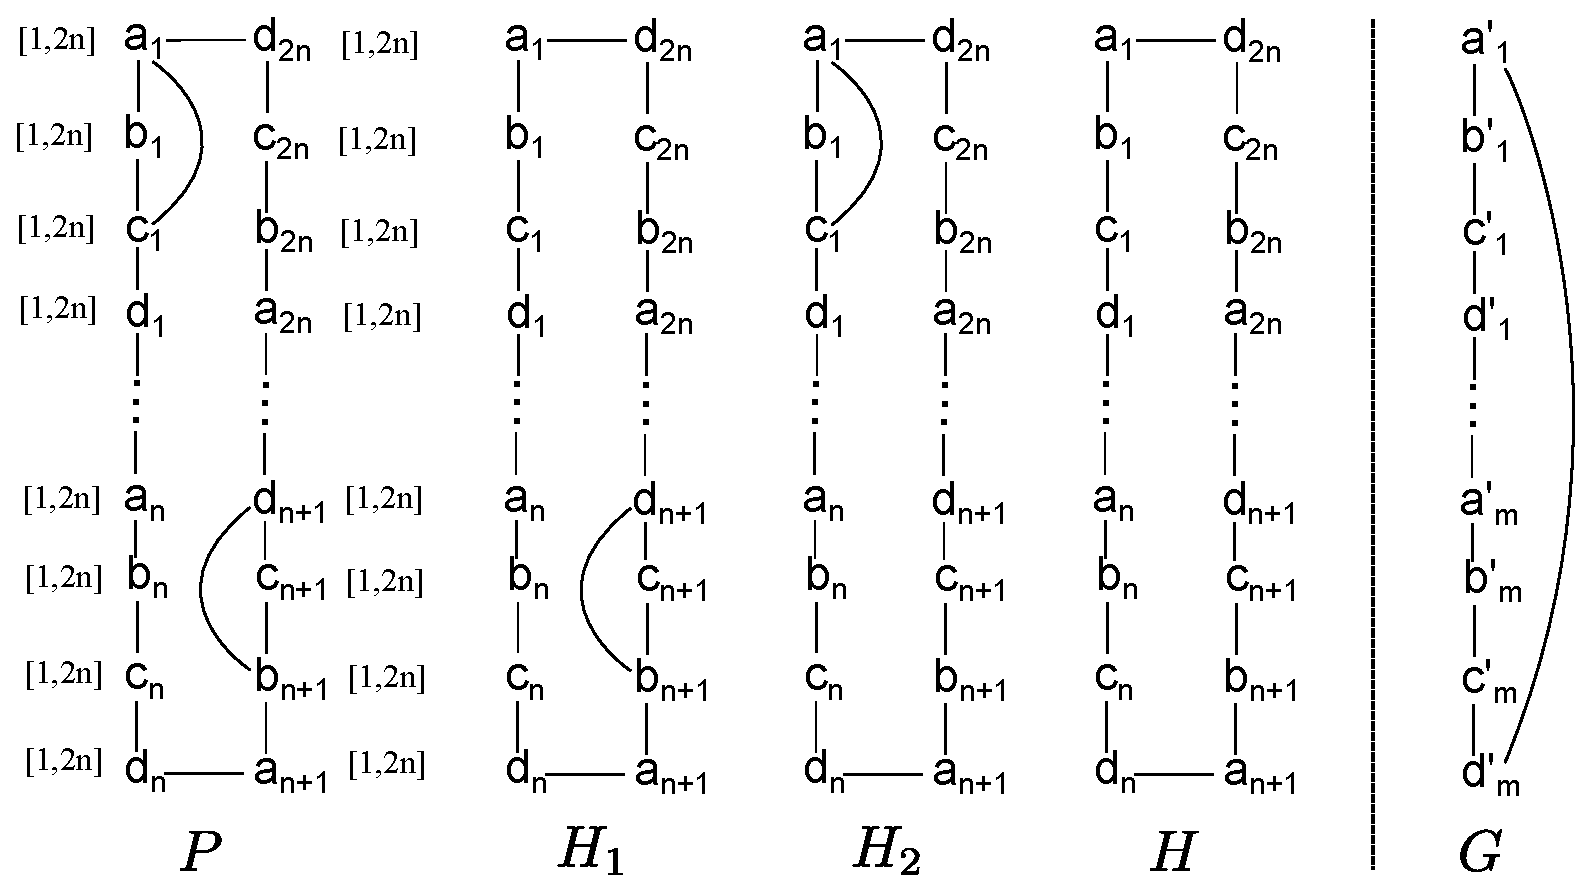
\includegraphics[scale=0.3]{./fig/inc-complexity-proof-pattern.eps}
\end{center}
\vspace{-3ex}
\caption{Unboundedness of single pattern update}
\vspace{-5ex}
\end{figure}

\etitle{(2) \dyngr is unbounded for single pattern update}.
Consider the following pattern and data graphs, and single pattern updates. Let data graph $G$ be a cycle ($a_1^G$, $b_1^G$, $c_1^G$, $d_1^G$, \ldots, $a_m^G$, $b_m^G$, $c_m^G$, $d_m^G$, $a_1^G$), where $a_i$, $b_i$, $c_i$ and $d_i$ have labels $A$, $B$, $C$ and $D$ respectively. Let pattern graph be a cycle ($a_1$, $b_1$, $c_1$, $d_1$, \ldots, $a_n$, $b_n$, $c_n$, $d_n$, $a_{n+1}$, $b_{n+1}$, $c_{n+1}$, $d_{n+1}$, \ldots, $a_{2n}$, $b_{2n}$, $c_{2n}$, $d_{2n}$, $a_1$) and two extra edges ($a_1$, $c_1$) and ($b_{n+1}$, $d_{n+1}$), where $a_i$, $b_i$, $c_i$ and $d_i$ have labels $A$, $B$, $C$ and $D$ respectively. Consider two single-edge deletions $\delta_1$ = ($a_1$, $c_1$) and $\delta_2$ = ($b_{n+1}$, $d_{n+1}$). Let $k = 1$ and $r$ = $4m$. Let $H_1$ and $H_2$ denote the graphs $P\oplus \delta_1$ and $P\oplus \delta_2$, respectively. Obviously, $PG_1(P, G) = PG_1(H_1, G) = PG_1(H_2, G) = \emptyset$, while $PG_1(H_1\oplus \delta_2, G) \neq \emptyset$. Assume that there exists a locally persistent incremental algorithm ${\cal A}$ for \dyngr. Let $Trace(P', \delta')$ denote the sequence of steps executed by the algorithm in processing some change $\delta'$ to some graph $P'$. Now consider the following two instances: the application of update $\delta_2$ to $P$ and the application of update $\delta_2$ to graph $H_1$. Obviously, the update procedure must behave differently in these two cases, and $Trace(P, \delta_2)$ must be different from $Trace(H_1, \delta_2)$ (because many vertices of $H_1\oplus \delta_2$ are affected, while no node in $P\oplus \delta_2$ is affected). Since a locally persistent algorithm makes use of no global storage, this can happen only both $Trace(P, \delta_2)$ and $Trace(H_1, \delta_2)$ include a visit to some node $w$ that contains different information in the graphs $P$ and $H_1$. However, $H_1$ was obtained from $P$ by applying change $\delta_1$. Hence the information at node $w$ must have been changed during the updating of applying $\delta_1$ to $P$. Therefore, $Trace(P, \delta_1)$ must also contain a visit to node $w$. As a characteristic of locally persistent algorithms is that if a vertex $w$ is visited during the updating of applying change $\delta'$ to graph $P'$, then every node in some path in $P'$ from a modified node of $\delta'$ to $w$ must have been visited.
Therefore, $Trace(P, \delta_1)$ and $Trace(P, \delta_2)$ both contain a visit to $w$, from the nodes in $\delta_1$ and $\delta_2$, respectively. Thus, $Trace(P, \delta_1)$ and $Trace(P, \delta_2)$ include visits to every node on some path from $a_1$ or $c_1$ to $b_{n+1}$ or $d_{n+1}$ respectively. Hence, the time taken for processing change $\delta_1$ to $P$ plus the time taken for processing change $\delta_2$ to $P$ must be no smaller than the distance between $a_1$ or $c_1$ to $b_{n+1}$ or $d_{n+1}$, \ie $n$, which is not a constant.
However, $|\kw{AFF}|$ in both cases are 1. Thus, the algorithm is not a bounded locally persistent incremental algorithm, which contradicts the assumption. That is, \dyngr is unbounded even for $k=1$ and single data update.

(1) and (2) together prove that \dyngr is unbounded even for $k=1$ and single pattern or data updates.


\subsection{Proof of Theorem~\ref{thm-fragmentation}}

The decision version of $\kw{OFGP}(P, m)$, denoted by $\kw{dOFGP}(P, m, r_1, r_2)$, is to decide whether there exists a fragmentation ${Pf}_1$, \ldots, ${Pf}_m$ and $F$ such that, (a) $\max_i |{Pf}_i| \leq r_1\cdot\frac{|P|}{m}$ and (b) $|F|\leq r_2|P|$.

\etitle{Upper bound}.
We show the \NP upper bound by providing an \NP algorithm to determine whether there exists an $m$-fragmentation of $P$. Given a pattern graph $P$, the algorithm works as follows.
\bi
\item Guess an $m$-fragmentation ${\cal P}_m$ of $P$;
\item check whether it satisfies restrictions of $r_1$ and $r_2$ (conditions (a) and (b) in the definition of decision problem $\kw{dOFGP}$, if so, return yes, otherwise go to the first step and guess another instance.
\ei

The algorithm is in \NP since step~2 can be checked in \PTIME (liner time, indeed).

\etitle{Lower bound}.
We next show that it is \NP-hard to determine whether there exists an $m$-fragmentation and remains \NP-hard even $m$ = 2, by reduction from the minimum cut problem, which is known \NP-complete\footnote{\small http://www.nada.kth.se/~viggo/wwwcompendium/node85.html}.

An instance of the minimum cut problem is given a undirected graph $H=(V,E)$ and a positive integer $k$, find a set $S \subseteq E$ of edges whose removal leaves two disjoint connected components, with $|S|\leq k$.

Given an instance of the minimum cut problem, we construct an instance of $m$-fragmentation problem, it can be achieved by taking $H$ as $P$, $m=2$, and setting $r_1=m$, $r2 = k/|P|$. Indeed, the minimum cut problem is a special case of the of $m$-fragmentation problem.



\subsection{Experiment}

\ni(1) {\em YouTube} provides a video network with video-video edges\footnote{\small http://netsg.cs.sfu.ca/youtubedata/} indicate recommendation relationships. We also used the undirected version of it, the edges between two videos indicate the correlate relationships. The dataset has 2,028,274 nodes and 12,218,972 edges, and we generated 403 labels according to the genre and age attributes of videos.

We generated the labels by the following routine. Each video in YouTube contains a set of attributes, \eg uploader, age, category, length. There are 13 categories in the data, and the age is calculated in terms of days. We classified the age into 31 periods, each contained 35 days. We then combined the period and the category attribute, get total 403 labels.


%\etitle{Multiple batch updates}. We secondly evaluated the performance of \optpatinc to process multiple batch updates. We fixed the number of hybrid unit updates in each batch update to be 3, and executed 5 batches one by one. We fixed the hybrid updates ratio with the same setting as in the hybrid updates experiment. X-axis represents the order of 5 batch updates, and Y-axis represents the elapsed time of each batch.
%
%The results are shown in Figures ~\ref{fig-exp-patinc-citation-multibatch}, ~\ref{fig-exp-patinc-youtube-multibatch} and ~\ref{fig-exp-patinc-synthetic-multibatch}. We find the following.
%(a) \optpatinc improves \grouprec by 12\% on on Citation and YouTube, 15\% on synthetic data in average for all batches.
%(b) The time increases with the coming of batch updates, while still pertains high efficiency in returning top-$k$ results. This justifies the effectiveness of {\em lazy update manner} developed in Section~\ref{subsubsec-affball}. Note that the case the elapsed time of \optpatinc surpasses \grouprec did not happen here. This is because even when all balls are identified as \affballsx, \optpatinc need not to process all accumulated pattern updates for them.
%Due to {\em update planner}, \optpatinc had already processed part of pattern updates for the set of \affballsx identified in the previous batches.
%(c) The time taken by \optpatinc on the 3$th$ batch update is the highest and further decreased a lot from the 4$th$ batch update. This is because all balls are identified as \affballsx on the 3$th$ batch update and the accumulated pattern updates stored in {\em update planner} are all processed. This makes the number of \affballsx identified and the elapsed time taken by \optpatinc on the 4$th$ batch update less. These justifies the effectiveness of the incremental model for pattern changes we have developed.

The results are shown in Figures ~\ref{fig-exp-patinc-citation-impper}, ~\ref{fig-exp-patinc-youtube-impper} and ~\ref{fig-exp-patinc-synthetic-impper}. We find the following.
(a) \kw{Affected} significantly improves \kw{Baseline} for 5 kinds of updates, especially for single-insertion updates. For multiple batch updates, \kw{Affected} outperforms \kw{Baseline} by 38\%, 54\% and 77\% on Citation, YouTube and synthetic data.
(b) \kw{ElrReturn} improves \kw{Baseline} a lot, especially for single-deletion updates. This is because more pattern nodes/edges removed from patterns will yield more results, which will enhance the pruning power.
(c) By utilizing the two techniques together, \grouprec outperforms \kw{Baseline} by 40\%, 56\% and 77\% on Citation, YouTube and synthetic data for multiple batch updates.



%\begin{figure*}[tb!]
%%\vspace{-2ex}
%\begin{center}
%
%\hfill
%\subfigure[{\small Real-life matches on Citation}]{\label{fig-exp-1-effect-citation}
%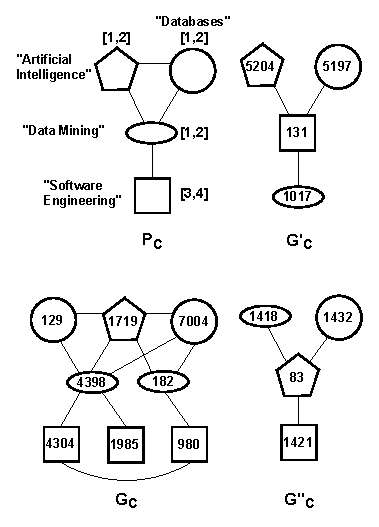
\includegraphics[scale=0.88]{./fig/exp-real-match-citation.eps}}
%\hfill
%\subfigure[{\small Vary $P$ (Citation)}]{\label{fig-exp-semantic-citation-density}
%\includegraphics[scale=0.39]{./fig/citation-semantic-density.eps}}
%\hfill
%\subfigure[{\small Vary $P$ (Citation)}]{\label{fig-exp-semantic-citation-capacity}
%\includegraphics[scale=0.39]{./fig/citation-semantic-capacity.eps}}
%\hfill
%\vspace{-2.5ex}
%
%\hfill
%\subfigure[{\small Vary $P$ (Citation)}]{\label{fig-exp-semantic-citation-link}
%\includegraphics[scale=0.39]{./fig/citation-semantic-link.eps}}
%\hfill
%\subfigure[{\small Vary $k$ (Citation)}]{\label{fig-exp-semantic-citation-density-varyk}
%\includegraphics[scale=0.39]{./fig/citation-semantic-density-varyk.eps}}
%\hfill
%\subfigure[{\small Vary $k$ (Citation)}]{\label{fig-exp-semantic-citation-capacity-varyk}
%\includegraphics[scale=0.39]{./fig/citation-semantic-capacity-varyk.eps}}
%\hfill
%\subfigure[{\small Vary $k$ (Citation)}]{\label{fig-exp-semantic-citation-link-varyk}
%\includegraphics[scale=0.39]{./fig/citation-semantic-link-varyk.eps}}
%\hfill
%\vspace{-2.5ex}
%
%\end{center}
%\vspace{-2.5ex}
%\caption{Performance evaluation of top-$k$ team formation semantic}
%\label{exp-semantic-effectiveness} \vspace{-2ex}
%\end{figure*}
%
%
%\begin{figure*}[tb!]
%%\vspace{-2ex}
%\begin{center}
%
%\hfill
%\subfigure[{\small Vary deletions (Citation)}]{\label{fig-exp-patinc-citation-del}
%\includegraphics[scale=0.314]{./fig/citation-pattern-deletion.eps}}
%\hfill
%\subfigure[{\small Vary insertions (Citation)}]{\label{fig-exp-patinc-citation-ins}
%\includegraphics[scale=0.314]{./fig/citation-pattern-insertion.eps}}
%\hfill
%\subfigure[{\small Vary capacity (Citation)}]{\label{fig-exp-patinc-citation-cap}
%\includegraphics[scale=0.314]{./fig/citation-pattern-capchange.eps}}
%\hfill
%\subfigure[{\small Vary hybrid updates (Citation)}]{\label{fig-exp-patinc-citation-hyb}
%\includegraphics[scale=0.314]{./fig/citation-pattern-hybrid.eps}}
%\hfill
%\subfigure[{\small Vary workloads (Citation)}]{\label{fig-exp-patinc-citation-multibatch}
%\includegraphics[scale=0.314]{./fig/citation-pattern-multi.eps}}
%\hfill
%\vspace{-2.5ex}
%
%\end{center}
%\vspace{-4ex}
%\caption{Performance evaluation of pattern incremental algorithms}
%\label{exp-patinc-efficiency} \vspace{-2ex}
%\end{figure*}
%
%
%\begin{figure*}[tb!]
%%\vspace{-2ex}
%\begin{center}
%
%\hfill
%\subfigure[{\small Vary data deletions (Citation)($\times 10^{4}$)}]{\label{fig-exp-datainc-citation-del}
%\includegraphics[scale=0.395]{./fig/citation-data-deletion.eps}}
%\hfill
%\subfigure[{\small Vary data insertions (Citation)($\times 10^{4}$)}]{\label{fig-exp-datainc-citation-ins}
%\includegraphics[scale=0.395]{./fig/citation-data-insertion.eps}}
%\hfill
%\subfigure[{\small Vary data hybrid updates (Citation)}]{\label{fig-exp-datainc-citation-hyb}
%\includegraphics[scale=0.395]{./fig/citation-data-hybrid.eps}}
%\hfill
%\subfigure[{\small Vary degree 1 (Synthetic)}]{\label{fig-exp-patinc-citation-multiworkload}
%\includegraphics[scale=0.395]{./fig/citation-pattern-multi.eps}}
%\hfill
%\vspace{-2.5ex}
%
%\end{center}
%\vspace{-4ex}
%\caption{Performance evaluation of data incremental algorithms}
%\label{exp-datainc-efficiency} \vspace{-2ex}
%\end{figure*}


%\etitle{Techniques comparison}. In this set of experiments we evaluated the effectiveness of (1)
%{\em affected balls identification}, and (2) {\em early-return strategy}. We implemented another three algorithms: (a) \kw{Baseline}, update $\tilde{M}(P,G)$ for all pattern updates and all balls in $G$; (b) \kw{Affected}, incorporating {\em affected balls} into \kw{Baseline}; (c) \kw{ElrReturn}, incorporating {\em early-return strategy} into \kw{Baseline}. Along with \grouprec, incorporating both {\em affected balls} and {\em early-return strategy} into \kw{Baseline}, we test to see the improved percentage of \kw{Affected}, \kw{ElrReturn} and \grouprec compared with \kw{Baseline}.


\subsection{To Read}

\stitle{Space analysis of all auxiliary structures}.

\etitle{Fragment-ball status index}. The time to construct Fragment-ball status index is bounded by $O(2^hh)$, and the storage space is $2^hh$, which is small compared to $G$ ($h$ is typically small, \eg 3 or 4, as shown in Section~\ref{sec-expt}). The index does not change during the following incremental process.

\etitle{Ball status index}. The time to construct Fragment-ball status index is bounded by $O(|V|)$, and the storage space is $3V$. The time to maintain the index is bounded by $O(||\affballsx||)$ ($||\affballsx||$ denotes the number of \affballsx). As it need to update the match status, \cflag and optional density bound \dens of each \affballx, after the incremental computation on partial match results.

\etitle{Fragment-ball matches}. The time to construct Fragment-ball matches is bounded by $O(|P|\Sigma_{v\in G}|\ball{v, r}|)$, and the storage space is $|P|\Sigma_{v\in G}|\ball{v, r}|$. Due to the cubic complexity, we adopt the storage strategy to bound the storage consumption within $|G|$. Given pattern update $\Delta P$ and data update $\Delta G$, the time to maintain the fragment-ball matches is bounded by $O(\bigcup_{\widehat{G\oplus\Delta G}\in \affballsx}(|\Delta P||M(P, \hat{G})|^2 + |P \oplus \Delta P||\affballsx|)$. Indeed, the time to maintain fragment-ball matches by refining on previous stored matches in processing certain updates in $\Delta P$ is bounded by $O(\bigcup_{\widehat{G\oplus\Delta G}\in \affballsx}(|\Delta P||M(P, \hat{G})|^2)$, and the time to maintain fragment-ball matches by recomputing matches in in processing certain updates $\Delta P$ and all updates in $\Delta G$ is bounded by $O(\bigcup_{\widehat{G\oplus\Delta G}\in \affballsx}(|P \oplus \Delta P||\affballsx|)$


\etitle{Ball filtering code}. The time to construct ball filtering code is bounded by $O(2^hh)$, and the storage space is $2^hh$. Given pattern update $\Delta P$, the time to maintain the code is in $O(2^h|\Delta P|)$. As for each single pattern update, the incremental process changes at most all $2^h$ type codes in the ball filtering code.

\etitle{Update planner}. The update planner is empty at beginning of the incremental process, it records the id of all single pattern updates. Given pattern update $\Delta P$, the time to maintain it is bounded by $O(|\Delta P|)$, and the storage space is $|\Delta P|$.

In summary, by storing the fragment-ball matches within storage size bound $|G|$, it can be assured the total size of auxiliary structure is $2^{h+1}h+|G|+3|V|+|\Delta P|$.

The time to construct them is bounded by $O(2^{h}h+|P|\Sigma_{v\in G}|\ball{v, r}|)$, and the time to maintain it is bounded by $O(\bigcup_{\widehat{G\oplus\Delta G}\in \affballsx}(|\Delta P||M(P, \hat{G})|^2 + |P \oplus \Delta P||\affballsx|)+2^h|\Delta P|)$


In the experiment, we find that at beginning of the incremental process, it takes 17MB and 120MB to store fragment-ball status index, ball status index and ball filtering code on Citation and synthetic data, compared to 36MB and 482MB to store the entire data graph. For storing fragment-ball matches, whose space complexity is rather higher, however, in practice, it cannot have that much matches due to the constraints carried by pattern graphs. It only takes 6MB and 4MB to store fragment-ball matches on Citation and synthetic data.



\stitle{The Facebook and Twitter statistics}.

We have conducted a survey on real-life network. The user increments on Facebook\footnote{\small http://www.statista.com/statistics/264810/number-of-monthly-active-facebook-users-worldwide/} and Twitter \footnote{\small http://www.statista.com/statistics/282087/number-of-monthly-active-twitter-users/} network daily reaches 1.23\textperthousand\ and 2.47\textperthousand. According to the statistics before, \datainc can process much more than 10\% increments at a high efficiency, which means \datainc can process the increments efficiently accumulated in 40 days and 81 days on Facebook and Twitter.


\stitle{The running example on incremental problem}.

\begin{example}
\label{exm-pattern-challenge-cp}
Consider pattern graph $P_1$ (without dashed lines) and data graph $G_1$ of Fig.~\ref{exm-motivation}, and fix $r=2$. When set $k=|V_{G_1}|=24$, meaning $PG_k(P,G)$ = $PG(P,G)$, \ie we have all perfect subgraphs as input for incremental process, that is the one resides in $\ball{SA_1, 2}$ and the other one in $\ball{SA_2, 2}$. For simplicity, we only consider the case there are no matched subgraphs in $G_1$, that satisfy the structural constraints but pruned by capacity constraints. We set $k'=1$, meaning we only want to find top-1 perfect subgraph in updated $P_1$ and $G_1$.

(1) When a pattern update comes, containing only an edge delete $(\kw{SD},\kw{ST})^-$, which will turn more unmatched nodes to matched. $\ball{SA_1, 2}$ and $\ball{SA_2, 2}$ certainly contain matches for the updated pattern structure but need recomputed for new matched nodes and further capacity constraint check. For all the other balls, the update will introduce matches within them and we need to compute for all.

(2) When a pattern update comes, containing only an edge insert $(\kw{BA},\kw{UD})^-$, which will turn matched nodes to unmatched, it means the balls do not have matches for $P$ will not have matches for the updated pattern graph. Therefore, we can get updated subgraphs by incremental computation on the results in $\ball{SA_1, 2}$ and $\ball{SA_2, 2}$.

(3) When a pattern update comes, containing only a capacity change on pattern node $\kw{UD}$, the lower bound changes from 1 to 2. We can get updated subgraphs by checking the results in $\ball{SA_1, 2}$ and $\ball{SA_2, 2}$.

(4) Consider another case when a data edge delete $(\kw{UD_5},\kw{ST_4})^-$ comes, which will turn matched nodes to unmatched. We need to identify the balls that are affected by the data changes, which can be time-consuming. However, if a ball do not have matches for $P$ in $G$, it cannot have matches for $P$ in the updated $G$, and do not need to check for new results.

(5) Consider another case when a data edge insert $(\kw{PM_3},\kw{BA_3})^+$ comes, which will certainly introduce new matches. We need to identify the balls that are affected by the data changes. Unlike the delete case, no matter a ball have matches or not for $P$ in $G$ may have matches for $P$ in the updated $G$, and should be checked for new results.



\end{example}



{\bf Section 3}:

In light of the challenges, we propose a unified incremental framework for $\dyngr$.
By designing novel auxiliary structures, the framework effectively localizes the impacts of pattern and data changes by (a) decomposing the maximum match relation $M(P, G)$ \wrt structure of pattern $P$ and balls in $G$, and (b) effectively restricting, localizing and locating impacts of changes to small parts of the decomposed $M(P,G)$.
More specifically, the structure contains two components: (1) {\em fragment-ball matches}, to achieve (a) decomposing and storing $M(P, G)$; and (2) index structures to achieve (b) identifying affected parts in the fragment-ball matches \wrt pattern and data changes.

The auxiliary structure is designed based on the following two observation.

\etitle{(1) The computation of graph simulation is decomposable}.
The computation of the match relation $R$ of a pattern $P$ in a data graph $G$ via graph simulation, which is the building block of $r$-simulation, is {\em decomposable} with {\em no overhead}. More specifically, we can compute $R$ in two phases:
we first break down $P$ into fragments $Pf_{1}$, \ldots, $Pf_{m}$, by removing a set $F$ of pattern edges; we then compute $R$ in two steps:
(a) computing match relation $R_{i}$ of $Pf_{i}$ in $G$ and (b) combining $R_{1}$, \ldots, $R_{m}$ into $R$ with $F$.
Indeed, both of the two steps can be implemented with the standard and fastest graph simulation algorithm~\cite{infsimu95}.
The benefit of this decomposed computation of $R$ is obviously: for any pattern changes, which has global impacts on $G$, we can restrict its impacts {\em within $R_{i}$}, where $R_{i}$ is the maximum match relation of $Pf_{i}$ in $G$. That is, instead of trying to recompute $R$ for $P$ and $G$ from scratch, by using $R_{1}$, \ldots, $R_{m}$, we can {\em control} the impacts of pattern changes, which are global with traditional approaches.
Moreover, this benefit comes with {\em no cost}. Indeed, let the computation cost (total steps) of steps (a) and (b) to be $C_{a}$ and $C_{b}$, and let $C$ be the cost of directly computing $R$ with $P$ and $G$, then by the nature of the graph simulation computation, one can verify that $C_{a} + C_{b} = C$, for any $P$, $G$ and any fragmentation $Pf_{1}$, \ldots, $Pf_{m}$ and $F$ of $P$.

This motivates us to store match relations with pattern fragments, instead of patterns as in conventional approaches. The framework makes use of this idea by maintaining the fragment-ball matches, which will be discussed later.

\etitle{(2) Impacts of pattern and data changes are localizable}.
Since the computation unit of $r$-simulation are balls of the data graph, and the impacts of pattern and data changes can be localized within those {\em affected balls}, who (a) are impacted by the changes and (b) have the possibility to contain match results. In other words, we only need to compute the new match relations in these affected balls. This gives us another dimension to localize the impacts of pattern and data changes, from the data graph perspective. The difficulty includes how to efficiently identify the affected balls, and how to update their match results \wrt pattern and data changes afterwards. This motivates us to devise index structures that organizes pattern fragments and balls effectively.


\begin{figure}[tb!]
\label{fig-framework}
\begin{center}
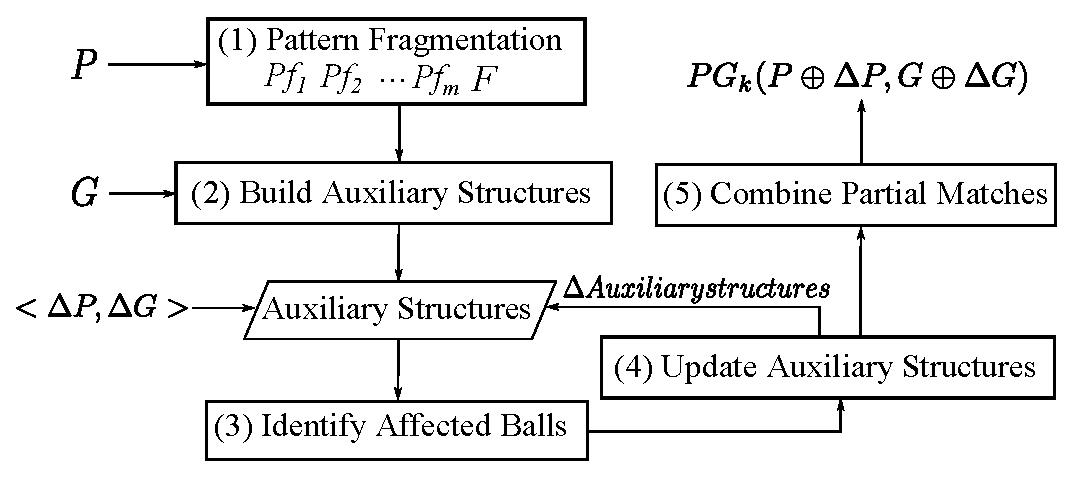
\includegraphics[scale=0.43]{./fig/inc-framework.eps}
\end{center}
\vspace{-3ex}
\caption{Incremental framework}
\vspace{-5ex}
\end{figure}

We are now ready to introduce the framework.

\stitle{Framework}. The framework, shown in Fig.~\ref{fig-framework}, consists of five components as follows.

\etitle{(1) Pattern fragmentation}, which breaks down the pattern graph into fragments while keeping its structure integrity.

\etitle{(2) Building auxiliary structures}, which initializes auxiliary structures to localize impacts of pattern and data changes.

\etitle{(3) Indentifying affected balls}, which makes use of the auxiliary structure to localizing the impacts.

\etitle{(4) Updating auxiliary structures}, which processes the auxiliary structure with pattern and data updates.

\etitle{(5) Combining partial results}, which combines processed partial matches to the final updated match results.


We below first present the auxiliary structures in Sections~\ref{subsubsec-fragmentation} and \ref{subsubsec-structure}. We then show how the framework handles the challenges with these structures in Section~\ref{subsubsec-handle}.

\subsubsection{Fragment-ball Matches}
\label{subsubsec-fragmentation}
We first discuss the pattern fragmentation (steps (1)) of the framework. Based on it, we then introduce the {\em fragment-ball match} structure.




\stitle{Fragment-ball matches}.
The {\em fragment-ball matches} $\tilde{M}(P,G)$ of pattern $P$ in data graph $G(V,E)$ \wrt $m$-fragmentation ${Pf}_1$, \ldots, ${Pf}_m$ is the set $\bigcup_{i\in[1,m], v\in V} M({Pf}_i, \ball{v,r})$, where $\ball{v,r}$ is the ball of $G$ with center $v$ and radius $r$, and $M({Pf}_i, \ball{v,r})$ is the maximum match relation of ${Pf}_i$ in ball $\ball{v,r}$.

Observe that, compared to $PG_k(P,G)$ or $M(P,G)$, $\tilde{M}(P, G)$ is much more informative to help localizing the impacts of pattern and data changes, and moreover, is of the same size asymptotically.



\subsubsection{Organizing Fragment-ball Matches}
\label{subsubsec-structure}

We next introduce the second part of the auxiliary structure, to organize the fragment-ball matches and to localize of impacts \wrt input changes.

\stitle{(1) Organize fragment-ball matches}.
Instead of storing fragment-ball matches $\tilde{M}(P, G)$ in a set, we organize $\tilde{M}(P, G)$ with two structures for the convenience of localizing the impacts in it.
More specifically, we use (a) {\em fragment-ball status index} and (b) {\em ball status index} to organize $\tilde{M}(P, G)$ in terms of the match status between balls and pattern fragments. We then link them to the fragment-ball matches, to form an integrated organization of $\tilde{M}(P, G)$, called {\em fragment-ball math struct}, denoted by \fb.

\etitle{Fragment-ball status index}. Given an $m$-fragmentation ${\cal P}_m$ of $P$, it consists of $2^m$ tuples of boolean values $(b_1, b_2, \ldots, b_m)$ that classify balls in $G$ \wrt ${\cal P}_m$, referred to as {\em type codes}, where each $b_i (i\in [1,m])$ is either 0 or 1,
such that, for each ball that are classified with type code $(b_1, b_2, \ldots, b_m)$, $b_i (i\in [1, m])$ is 1 if and only if $Pf_i$ has matches in it. Intuitively, it is to encode the match relationships between pattern fragments and balls, which will be used for organizing fragment-ball matches.


\etitle{Ball status index}. It consists of $|V_G|$ triples $(bid, cflag, den)$, where $bid$ is an integer recording the $id$ of a ball, $cflag$ is an integer recording the id of a pattern update , and $den$ is a natural number recording the density bound of the ball. The usage of $cflag$ and $den$ is illustrated in next section.

\etitle{Fragment-ball match struct} (\fb). We next link fragment-ball matches, fragment-ball status index and ball status index together, referred to as {\em fragment-ball match struct} and denoted by \fb, as follows.
For each type code $tc$ = $(b_{1}, \ldots, b_{m})$ in the fragment-ball status component, there is a link from $tc$ to a record in the ball status component for a ball $\ball{v,r}$ such that if $b_i$ is 1, then fragment ${Pf}_{i}$ of ${\cal P}_{m}$ has a match in $\ball{v,r}$, and we say that ball $\ball{v,r}$ is of type $tc$.
For each ball $\ball{v,r}$, there exists a pointer from the record of $\ball{v,r}$ in the ball status component to $M({Pf}_{i}, \ball{v,r}) (i\in [1, m])$ in $\tilde{M}(P,G)$, if it is associated to a type code $tc$ with $tc[i] = 1$, \ie $M({Pf}_{i}, \ball{v,r})$ is not empty.


\begin{example}
\label{exa-matchindex}
An example of \fbmatstruct is illustrated in Fig.~\ref{fig-auxstr-index}, with pattern graph $P_1$ (without dashed edges) and data graph $G_1$ in Fig.~\ref{exm-motivation}, $r=2$, $k=k'=2$, and $m=2$, \ie $P_1$ is divided into fragments $Pf_{1}$ and $Pf_{2}$ according to Algorithm \kw{PFrag} shown in Fig.~\ref{alg-PFrag}. \fbmatstruct consists of three parts: structure (i) the fragment-ball status index, structure (ii) the local status index and (iii) the fragment-ball matches.
In structure (i), there are $2^2=4$ type codes that classify balls of $G_1$ into 4 types.
For balls linked from type code (1, 1), \eg balls $\ball{\kw{SA_1},2}$ and $\ball{\kw{SA_2},2}$, there are matches to both $Pf_{1}$ and $Pf_{2}$ in them.
For balls connected to type code (1, 0), \eg ball $\ball{\kw{PM_2},2}$, as depicted in Fig.~\ref{exm-motivation}, the left part of the dashed vertical line (II) together with node \kw{SA_1} and the related edge. There exist matches for $Pf_{2}$, but no matches for $Pf_{1}$ in the ball.
For balls connected to type code (0, 1), \eg ball $\ball{\kw{SA_3},2}$, there exist matches for $Pf_{1}$, but no matches for $Pf_{2}$.
For balls connected to type code (0, 0), \eg ball $\ball{\kw{BA_3},2}$, there exist no match for either of $Pf_{1}$ or $Pf_{2}$. We only consider these 5 balls shown in the figure in the following.
\end{example}

\stitle{(2) Localizing impacts in fragment-ball matches}.
We next introduce the structure for identifying {\em affected balls}. We firstly give a formal definition of {\em affected balls} below. We then describe the structure, called {\em ball filtering code}.

\etitle{Affected balls}.
For any pattern $P$, $m$-fragmentation ${\cal P}_{m}$, data graph $G$, update $\Delta P$, update $\Delta G$, and fragment-ball matches $\tilde{M}(P,G)$,
we say a ball $\ball{v,r}$ is an {\em affected ball} \wrt $P$, ${\cal P}_{m}$, $G$, $\tilde{M}(P,G)$, $\Delta P$ and $\Delta G$, denoted by \affballx, if for any algorithm $\Gamma$
that takes as input $P$, ${\cal P}_{m}$, $G$, $\tilde{M}(P,G)$, $\Delta P$ and $\Delta G$,
and computes $P\oplus\Delta P(G\oplus\Delta G)$ by updating $\tilde{M}(P,G)$ in terms of balls, $\Gamma$ has to check for update in $M(P,\ball{v,r})$.
That is, \affballsx are balls of $G$ that have to be checked for update in {\em fragment-ball matches} by any correct pattern incremental algorithm in the presence of $\tilde{M}(P,G)$.


It is worth mentioned that a pattern edge/node insert will turn a matched node to unmatched, and a pattern edge/node delete will turn a unmatched node to matched.
Given a pattern fragmentation $Pf_{1}$, \ldots, $Pf_{m}$ of $P$, $\Delta P$ and a ball $\ball{v,r}$, if there exists a perfect subgraph in $\ball{v,r}$ for $P \oplus P$, then the following is true.
Suppose (1) $\Delta P$ contains (a) only an edge/node insert on $Pf_{1}$, (b) only a capacity change or (c) only an edge insert/delete on the cut edges, there exist (partial) matches for each fragment of $P$ in $\tilde{M}(P,G)$;
(2) $\Delta P$ contains only an edge/node delete on $Pf_{1}$, there exist (partial) matches for $Pf_{2}$, \ldots, $Pf_{m}$ of $P$ in $\tilde{M}(P,G)$;

The framework utilizes this idea to filter out balls cannot match with $P \oplus P$, based on the current partial match status, and regard the other candidate balls who may contain perfect subgraphs as {\em affected balls}. It restrict the pattern change impact from global to local, by turning the incremental computation for all balls to {\em affected balls} in $G$.


According to \fbmatstruct, all balls in $G$ are classified to $2^m$ types. For pattern update $\Delta P$, we will next present the auxiliary structure {\em ball filtering code} to identify \affballsx \wrt $\Delta P$, referred to as \ballfilter.
More specifically,  \ballfilter is used to encode whether $\Delta P$ causes a need to update $\tilde{M}(P,G)$ and further whether causes a visit to a ball in $G$.

\etitle{Ball filtering code} (\ballfilter).
Given an $m$-fragmentation ${\cal P}_{m}$ of pattern $P$, and $\Delta P$, \ballfilter for $P$ \wrt $\Delta P$ consists of $2^{m}$ tuples of $m$-bit boolean strings, referred to as {\em filtering codes}. They are all initially set to $fc=\underbrace{11\ldots 1}_{m}$, corresponding to a type code in {\em fragment-ball status index}, and are updated for all unit update $\delta$ in $\Delta P$:
(i) when $\delta$ is a single-node delete $(u)^{-}$ or a single-edge delete $(u_{1}, u_{2})^{-}$ to fragment ${Pf}_{i}$ of ${\cal P}_{m}$, the $i$-th bit of the ball filtering code for $P$ is set to 0; otherwise, (ii) \ballfilter remains unchanged.

For data update $\Delta G$, the ball based team formation semantic provides the convenience for localizing data change impacts, allowing us to find the set of affected balls, and only compute matches within them. The method to identify \affballsx \wrt $\Delta G$ involves some structural computation on $G$, which will be shown in in Section~\ref{sec-IncAlg}.

\begin{example}
\label{exa-ball-filtering-code}
An example of \ballfilter is illustrated in Fig.~\ref{fig-inc-maintain-unit}, with pattern graph $P_1$ and data graph $G_1$ in Fig.~\ref{exm-motivation}. The \ballfilter contains $2^{2}=4$ $2$-bit boolean strings and are all initialized to be $11$, as shown in the first column in the \ballfilter table. When a batch update $\Delta P_1$ comes, which contains one single update $\delta_1$, a single-edge deletion $(\kw{SD},\kw{ST})^-$, which is included in $Pf_{1}$. Thus all the 4 boolean strings change to 10, as shown in the second column.

Consider another case a batch update $\Delta P_5$ comes, which contains two single update $\delta_1$ and $\delta_2$, a single-edge deletion $(\kw{SD},\kw{ST})^-$ in $Pf_{1}$ and a single-edge insert $(\kw{BA},\kw{UD})^+$ in $Pf_{2}$. The \ballfilter changes as shown in the second column in Fig.~\ref{fig-inc-maintain-batch}, the 4 boolean strings are also 10, which is same with the former case as the edge insert does not change \ballfilter.

Consider the third case a data edge insert $(\kw{PM_3},\kw{BA_3})^+$ comes, the match results must be contained in (1) the balls with type code (1,1), and (2) the balls centered with $\kw{SA_3}$, $\kw{PM_3}$, $\kw{UD_4}$, $\kw{BA_3}$ and $\kw{UD_5}$. For (1), we only need to retrieve partial match results from $\tilde{M}(P,G)$ and compute to get final results; for (2), we need to access $G$ to update the partial results in $\tilde{M}(P,G)$ and further compute to get final results. The method to identify \affballsx for $\Delta G$ will be discussed later.
\end{example}



\eat{%%%%%%%%%%%
a triple $B_{i}(\checkflag,
\dens, \densityflag)$ for ball $B_{i}$ (suppose balls in $G$ are numbered from $1$ to $V$), such that, $B_{i}[\checkflag]$ recors which update in $\Delta P$ has been processed up by the last time when the $i$-th ball in $G$ is treated as an \affball when processing updates in $\Delta P$ one by one; $B_{i}[\dens]$ records the density of ball $B_{i}$, which will be used later to optimize the process of reusing results in $\tilde{M}(P,G)$; and $B_{i}[\densityflag]$ records a flag denoting whether we need to refresh the $B_{i}[\dens]$ or not.
For each type code $tc$ = $(b_{1}, \ldots, b_{m})$ in the fragment-ball status component, there is also a link from $c$ to records in the local status component for balls $B_{i}$ such that fragment $P_{i}$ of ${\cal P}_{m}$ has a match in $B_{i}$, and say that ball $B_{i}$ is of type $tc$.
For each ball $B_{i}$ ($i\in [1, |V|])$, there exists a pointer from the record of $B_{i}$ in the local status component to $M(P_{j}, B_{i}) (j\in [1, m])$ if it is associated to a type code $tc$ with $tc[P_{j}] = 1$, \ie
$M(P_{j}, B_{i})$ is not empty.
}%EAT%%%%%%%%%%%



%Based on ${\cal P}_{m}$ and $\tilde{M}(P,G)$, we are readily to define the notion of {\em affected balls} \wrt $\Delta P$ and $\Delta G$.



\stitle{Auxiliary structure storage principle}. One typically has a budget on the size of space that can be used for storing auxiliary structure. We set the space bound to $C\cdot |G|$, where $C$ is small.



%%%%%%%%%%%%%%%%%%%%%%%%%%%%%%%%%%%%%%%%%%%%%
\begin{figure*}[tb!]
\begin{center}
\hspace{-4ex}
\subfigure{\label{fig-auxstr-index}
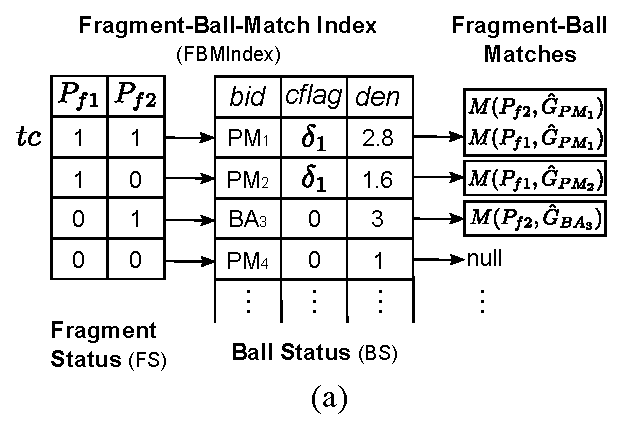
\includegraphics[scale=0.56]{./fig/fig-auxstr-index.eps}}
\subfigure{\label{fig-inc-maintain-unit}
\hspace{-1.5ex} \vrule \hspace{0.3ex} \hfill
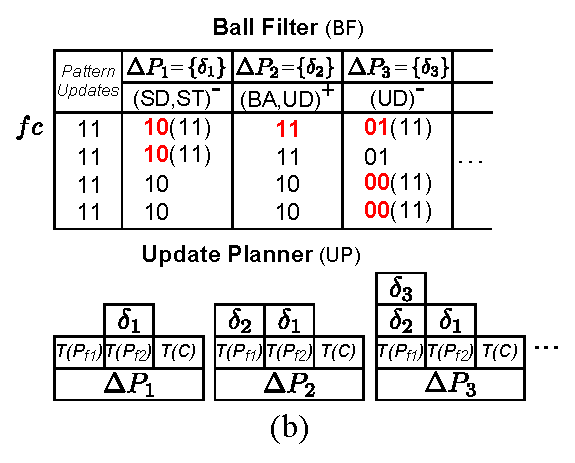
\includegraphics[scale=0.55]{./fig/fig-inc-maintain-unit.eps}}
\subfigure{\label{fig-inc-maintain-batch}
\hspace{-1.5ex} \vrule \hspace{0.3ex} \hfill
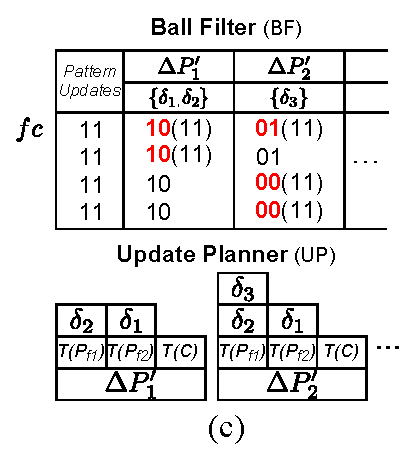
\includegraphics[scale=0.55]{./fig/fig-inc-maintain-batch.eps}}
\caption{Auxiliary data structures}
\label{fig-auxiliary-data-structures}
\end{center}
\vspace{-4ex}
\end{figure*}
%%%%%%%%%%%%%%%%%%%%%%%%%%%%%%%%%%%%%%%%%%%%%


\subsubsection{Handling challenges}
\label{subsubsec-handle}

With the auxiliary structures, the framework can achieve the following.
%, which solves the challenges raise at the beginning of the section.

\begin{theorem}
\label{thm-pattern-incremental}
For any pattern $P$, an $m$-fragmentation ${\cal P}_{m}$ of $P$, and data graph $G$,
with the auxiliary structure, there exists an incremental algorithm underlying the framework for \dyngr such that, for any batch update $(\Delta P, \Delta G)$, it can computes $(P\oplus \Delta P)(G\oplus \Delta G)$ in time determined by $P$, $\Delta P$, $\Delta G$, $\tilde{M}(P, G)$ and \affballx only, and is not directly dependent of $|G|$.
\end{theorem}

Based on this, below we discuss how the framework handles the challenges raised in Sectioin~\ref{subsec-challenges}. We prove Theorem~\ref{thm-pattern-incremental} by providing such algorithms in Section~\ref{sec-IncAlg}.

\sstab {\bf Solution (1): localizing changes impacts}. To solve challenge (1), the framework computes new matches in a ``{\em global-to-local}'' way with \fb and \ballfilter structures.

\sstab (I) for $\Delta P$, by storing $\tilde{M}(P,G)$ and the indexes in \fbmatstruct, it changes the problem of updating $PG_k(P,G)$ or $M(P,G)$ for $\Delta P$ to $P$, into updating $M({Pf}_i, G)$ for fragments ${Pf}_i$ to which $\Delta P$ apply, and then merging all $M({Pf}_i, G)$ together to $M(P\oplus \Delta P, G)$, which gives $PG(P\oplus \Delta P, G)$. This process localize the pattern change impacts from the whole patterns to pattern fragments.

\sstab (II) for $\Delta P$/$\Delta G$, by identifying \affballsx, it changes the problem of updating $\tilde{M}(P,G)$ for each ball in $G$, into updating $\tilde{M}(P, \ball{v,r})$ only within the set of \affballsx, and then merging all $M({Pf}_i, \ball{v,r})$ together to $M(P\oplus \Delta P, G\oplus \Delta G)$ within \affballsx, which gives $PG(P\oplus \Delta P,G\oplus \Delta G)$. This process localizes the pattern and data change impacts only to the related balls that may contain {\em new} match results \wrt $P$, $G$, \fbmatstruct, $\Delta P$ and $\Delta G$.

These two techniques restrict the pattern and data change impacts to those updated pattern fragments and the set of related balls in $G$, instead of entire $P$ and $G$. As will be shown later, this process theoretically effectively reduces the computation cost when compared to computing from scratch or computing from $M(P,G)$ directly via conventional unbounded incremental algorithms.


\sstab {\bf Solution (2): informative auxiliary data structures and space budget storage method}.

\sstab (I) To solve the problem what information to store in challenge (2), the framework maintains the {\em fragment-ball matches} $\tilde{M}(P,G)$,
 which has the following advantages compared to store $PG_k(P,G)$ directly as conventional incremental algorithms, or store $M(P,G)$ as some pattern incremental algorithms ~\cite{FanWW13-tods}.
 (i) On one hand, by the nature of graph simulation based algorithms~\cite{infsimu95}, the partial match relations $M({Pf}_i, \ball{v,r})$ in $\tilde{M}(P,G)$ are actually intermediate results for computing $M(P,\ball{v,r})$ (and thus $PG_k(P,G)$), which do not incur higher maintenance cost than maintaining $PG_k(P,G)$ as conventional incremental algorithms.
(ii) On the other hand, $\tilde{M}(P,G)$, together with $P$, is more informative than $PG_k(P,G)$ and even $M(P,G)$, as both $PG_k(P,G)$ and $M(P,G)$ can be naturally derived from $\tilde{M}(P,G)$ and $P$ by conducting graph simulation algorithms over $\tilde{M}(P,G)$ without additional computation cost, \ie $O(C_{\tilde{M}(P,G)} + C_{\tilde{M}\ra M}) = O(C_{M(P,G)})$, where $C_{\tilde{M}(P,G)}$ is the cost of computing $\tilde{M}(P,G)$ from $P$ and $G$, $C_{\tilde{M}\ra M}$ is the cost of computing $M(P,G)$ from $\tilde{M}(P,G)$ and $P$, and $C_{M(P,G)}$ is the cost of computing $M(P,G)$ directly from $P$ and $G$.


\sstab (II) To solve the problem on how to store information with space budget in challenge (2), the framework obeys the storage principle proposed above to store all auxiliary structures.
Moreover, the size of the auxiliary structure is not an overhead, as its size is comparable to the size of the match relation $M(P, G)$ of $P$ in $G$, which has anyway to be stored in the process of computing of $PG_{k}(P, G)$.
More specifically, observe that the total size of the auxiliary structures is $O(|\Sigma_{Pf\in {\cal P}_{m}}\Sigma_{v\in G}|Pf||\ball{v,r}|)$ + $C_{m}$ = $O(|P|\Sigma_{v\in G}|\ball{v,r}|)$ + $C_{m}$, where $C_{m}$ = $2^{m}$ is small compared to $G$ ($m$ is typically small, \eg 3 or 4, as shown in Section~\ref{sec-expt}). Observe that the match relation $M(P, G)$ is also of size $O(|P|\Sigma_{v\in G}|\ball{v, r}|)$, which has to be stored in the computation of $PG_{k}(P, G)$.


%\textbf{Space analysis of all auxiliary structures: the space of $\tilde{M}(P,G)$ is bounded by $O(|V||P||G|)$, two indexes: $O(|2^m+V_G|)$, ballfiltercode: $O(2^m)$.. the time of construct $\tilde{M}(P,G)$ is $O(|V||P||G|)$, two indexes: $O(|2^m+V_G|)$, ballfiltercode: $O(2^m)$.}


Despite of this, we next show how to, given a pattern graph $P$, a data graph $G(V,E)$, a size bound factor $C$ and an $m$-fragmentation $({Pf}_1, \ldots, {Pf}_m, F)$ of $P$,  construct $\tilde{M}^{C}(P,G)$ of size no larger than $C|G|$. Remember that $\tilde{M}(P,G)$ is the set $\bigcup_{i\in[1,m], v\in V} M({Pf}_i, \ball{G}[v,r])$. We below show how to pick a subset $\tilde{M}^C(P,G)$ of $\tilde{M}(P,G)$ such that the chances that $\tilde{M}^C(P,G)$ can best support our incremental approach.
To do this, we first define a ranking function that assigns scores to balls in $G$. We then show how to maintain the bounded size $\tilde{M}^{C}(P,G)$ through the whole computation.

\etitle{Ranking function}.
Given a data graph $G$, an $m$-fragmentation ${\cal P}_m$, we define a ranking function $\rho(\cdot)$ satisfying the following.
For each ball $\ball{v,r}$, $\rho(\ball{v,r})$ is a $(h, s)$, where $h\in [1, m]$ is an integer, $s$ is a real number, such that
\bi
\item [(i)] there are $h$ fragments in ${\cal P}_m$ to which $P$ matches;
\item [(ii)] $s = \dfrac{h}{\sum_{i\in [1,m]} |M(Pf_i, \ball{v,r})|}$.
\ei

Given two balls $\ball{v,r}$ and $\ball{v',r}$, we say $\ball{v,r}$ is ranked higher than $\ball{v',r}$ \wrt $\rho(\cdot)$, if
\bi
\item [(1)] $h_v > h_{v'}$; {\bf or}
\item [(2)] $h_v = h_{v'}$ and $s_v > s_{v'}$,
\ei
where $\rho(\ball{v,r}) = (h_v, s_v)$ and $\rho(\ball{v',r}) = (h_{v'}, s_{v'})$.

Intuitively, $\ball{v,r}$ ranks higher than $\ball{v', r}$ when (1) there are more pattern fragments matches $\ball{v,r}$ than $\ball{v',r}$, this is because the more pattern fragments have matches in a ball, the higher possibility it has a perfect subgraph with the updated $P$ and $G$; (2) If the number of fragments matches the two are equal, but it takes smaller space to store partial match relations of fragments in $\ball{v,r}$ than in $\ball{v',r}$, we adopt this method because with the equal space budget, it contains more information and can store more partial matches in terms of balls, surely reducing the computation work on computing balls and partial matches in the following incremental process.


\etitle{Maintaining $\tilde{M}^C(P,G)$}.
We next describe how to maintain $\tilde{M}^C(P,G)$. We processes balls of $G$ one by one. For each ball $\ball{v,r}$, we computes its ranking score $(h_v, s_v)$ by the ranking function $\rho(\cdot)$ defined above.
If there are enough space to store partial match relations in $\ball{v,r}$ in $\tilde{M}^C(P,G)$ within the space budget $C|G|$, we put it into $\tilde{M}^C(P,G)$. Otherwise, we check whether there are balls whose partial match relations are stored in $\tilde{M}^C(P,G)$ but rank lower than $\ball{v,r}$. If the total size of partial match relations in these balls is larger than that in $\ball{v,r}$, we then replace partial match relations in the lowest ranked balls in $\tilde{M}^C(P,G)$ with the ones in $\ball{v,r}$ instead. If no such balls found, then we do not put partial match relations in $\ball{v,r}$ into $\tilde{M}^C(P,G)$.



\sstab {\bf Solution (3): support for both pattern and data graph changes}. The unified framework can process pattern and data changes together or in any arbitrary order. This is because for pattern or data updates, the framework processes them following the same routine. More specifically,

\sstab (I) the framework constructs the same auxiliary structures \fbmatstruct for incremental computation;

\sstab (II) for either $\Delta P$, $\Delta G$ or $\Delta P$ and $\Delta G$ together, the incremental process identifies \affballsx by taking the union of \affballsx \wrt $\Delta P$ and \affballsx \wrt $\Delta G$.

\sstab (III) for the set of \affballsx, the incremental process updates the partial results in $\tilde{M}(P,G)$ and maintains the other auxiliary structures \wrt $\Delta P$ and $\Delta G$. It then combines the updated partial results to get the final match results.


{\bf Section 4}:

\stab
\etitle{(1) Updating update planner and \ballfilter}. When a batch update $\Delta P$ arrives, the update planner is updated by processing all unit updates in $\Delta P$ in an ascending order by their update IDs. \ballfilter is also updated \wrt $\Delta P$.

\stab
\etitle{(2) Identifying \affballsx}. \patinc then invokes \identifyaffball to identify \affballsx due to the arrival of $\Delta P$.

\stab
\etitle{(2) Compute partial match relations in \affballsx}. For each ball $\ball{v,r}$ that is marked as \affballx, for each pattern fragment ${Pf}_i$, computes $M({Pf}_i\oplus \Delta {Pf}_i, \ball{v,r})$ from $M({Pf}_i, \ball{v,r})$ by using the methods which will proposed in Section~\ref{subsubsec-ball}, where $\Delta {Pf}_i$ consists of all unit updates stored in $T({Pf}_i)$ with update IDs larger then $\ball{v,r}[\cflag]$ in \matchindex.

\stab
\etitle{(4) Combining partial match relations}. \patinc then uses the method which will proposed in Section~\ref{subsubsec-merge} to merge $M({Pf}_i\oplus \Delta {Pf}_i, \ball{v,r})$ computed above for all \affballsx along with updates in $T(F)$ to the cut $F$ of $P$. \patinc outputs the top-$k$ results of this step as answers to the current batch update received.

\stab
\etitle{(5) Updating \matchindex}. To handle future batch updates, \patinc also updates \matchindex by setting $\ball{v,r}[\cflag]$ to $\kw{id}_\delta$ for each ball $\ball{v,r}$ marked as \affballx. \patinc then checks on the match status of the ball according to $M({Pf}_i\oplus \Delta {Pf}_i, \ball{v,r})$ and updates the link from the corresponding type code $tc$ in fragment-ball status component to the record of $\ball{v,r}$ in the ball status component. \patinc finally sets all balls non \affballsx at the end and reset the corresponding $fc$ in \ballfilter of \affballsx to 11.


%%%%%%%%%%%%%%%%%%%%%%%%%%%%%%
\stitle{Remark}. When $\Delta P$ contains a node-insert update with new label on the node, the density upper bound stored in $\ball{v,r}[\kw{den}]$ for each ball $\ball{v,r}$ needs to be refreshed as Step (1) of the linear approximation algorithm has to be recomputed. We handle this by
(i) extending the ball status component of \matchindex for each ball $\ball{v,r}$ with a new field called \dflag, which is a natural number that indicates whether the density of a ball needs to be refreshed; and
(ii) extending the fragment-ball status component of \matchindex for each match status with a new field called \rflag, which is a natural number that decides whether the density upper bound of all balls of the current type code are updated (omitted).
With these, algorithm \optpatinc is able to
\bi
\item [(a)] determine whether $\ball{v,r}[\kw{den}]$ needs update for each \affballx $\ball{v,r}$ in $O(1)$ time; and
\item [(b)] decide whether the density upper bounds of all \affballsx are updated within $O(2^m)$ time ($m$ is the number of fragment of pattern $P$ and is typically very small), {\em independent of the number of \affballsx}.
\ei

%%%%%%%%%%%%%%%%%%%%%%%%%%%%%%

\subsubsection{Bounded Storage Principle}


In summary, the space of the entire auxiliary structures is $2^{h+1}h+ \sizeof(fbm)+3|V|+|\Delta P|$.  One typically has a budget on the size of space that can be used for storing auxiliary structure. We set the space bound to $\sizeof(fbm)\le \sizeof(G)$, where $C$ is small.

In the experiment, we find that at beginning of the incremental process, it takes 17MB and 120MB to store fragment-ball status index, ball status index and ball filtering code on Citation and synthetic data, compared to 36MB and 482MB to store the entire data graph. For storing fragment-ball matches, whose space complexity is rather higher, however, in practice, it cannot have that much matches due to the constraints carried by pattern graphs. It only takes 6MB and 4MB to store fragment-ball matches on Citation and synthetic data.

\stitle{Ranking based space bounding policy}.
Given a data graph $G$, an $m$-fragmentation ${\cal P}_m$, we define a ranking function $\rho(\cdot)$ satisfying the following.
For each ball $\ball{v,r}$, $\rho(\ball{v,r})$ is a $(h, s)$, where $h\in [1, m]$ is an integer, $s$ is a real number, such that
\bi
\item [(i)] there are $h$ fragments in ${\cal P}_m$ to which $P$ matches;
\item [(ii)] $s = \dfrac{h}{\sum_{i\in [1,m]} |M(Pf_i, \ball{v,r})|}$.
\ei

Given two balls $\ball{v,r}$ and $\ball{v',r}$, we say $\ball{v,r}$ is ranked higher than $\ball{v',r}$ \wrt $\rho(\cdot)$, if
\bi
\item [(1)] $h_v > h_{v'}$; {\bf or}
\item [(2)] $h_v = h_{v'}$ and $s_v > s_{v'}$,
\ei
where $\rho(\ball{v,r}) = (h_v, s_v)$ and $\rho(\ball{v',r}) = (h_{v'}, s_{v'})$.

Intuitively, $\ball{v,r}$ ranks higher than $\ball{v', r}$ when (1) there are more pattern fragments matches $\ball{v,r}$ than $\ball{v',r}$, this is because the more pattern fragments have matches in a ball, the higher possibility it has a perfect subgraph with the updated $P$ and $G$; (2) If the number of fragments matches the two are equal, but it takes smaller space to store partial match relations of fragments in $\ball{v,r}$ than in $\ball{v',r}$, we adopt this method because with the equal space budget, it contains more information and can store more partial matches in terms of balls, surely reducing the computation work on computing balls and partial matches in the following incremental process.
